\documentclass{article}
%\usepackage[a4paper, total={6in, 8in}]{geometry}
\usepackage{geometry}
 \geometry{
 a4paper,
 total={210mm,297mm},
 left=20mm,
 right=20mm,
 top=-2mm,
 bottom=2mm,
 }
 
\usepackage[utf8]{inputenc}
\usepackage{graphicx}
%\usepackage[margin=0.5in]{geometry}

\usepackage{amsmath,amssymb}
\usepackage{ifpdf}
%\usepackage{cite}
\usepackage{algorithmic}
\usepackage{array}
\usepackage{mdwmath}
\usepackage{pdfpages}
\usepackage{mdwtab}
\usepackage{eqparbox}
\usepackage{cite}
%\onecolumn
%\input{psfig}
\usepackage{color}
\usepackage{graphicx}
\setlength{\textheight}{23.5cm} \setlength{\topmargin}{-1.05cm}
\setlength{\textwidth}{6.5in} \setlength{\oddsidemargin}{-0.5cm}
\renewcommand{\baselinestretch}{1}
\pagenumbering{arabic}
\usepackage{ragged2e}
\renewcommand{\baselinestretch}{1.5}

\begin{document}

\textbf{
\begin{center}
{
\large{School of Engineering and Applied Science (SEAS), Ahmedabad University}\vspace{4mm}
}
\end{center}
%
\begin{center}
\large{B.Tech(ICT) Semester IV: Probability and Random Processes (MAT 202) }\\ \vspace{3mm}
\end{center}
}
\begin{itemize}
\item \textbf{Project Title: \textit{ Alzheimer Disease Prediction Model}}
\item Group No : $H\_B33$
\item Name (Roll No) :  
\begin{enumerate}
    \item Parth N Patel  \hspace{0.8cm} (AU1841028)
    \item Shivam Lakhtariya \hspace{0.10cm} (AU1841084)
\end{enumerate}
%\item Roll no: s1749002 (Ph.d)
%\item Associated with Project: DST-UKIERI


\end{itemize} 

\section{Introduction}
\subsection{Background}
Alzheimer’s disease is also known as a disease of Old Age. There is no specific drug to cure Alzheimer's Disease(AD) or to slowdown it. Generally AD is caused between age of 60-75 years. A Recent discovery had shown that the presence of $\epsilon$4\cite{1} of the ApoE Gene indicates the presence of the onset of Alzheimer Disease.
\\ The Presence of AD Diseases can be known by the following facts:
\begin{enumerate}
    \item Large Amount of Deposits of $\beta$-amyloid protien
    \item Neurofibrillary tangles (connections between neurones)
    \item Amyloid Protien in the arteries of brain.
    \item Loss of Neurones
\end{enumerate}
AD is the most commonest form of cognitive impairement, it is hard to diagnose AD with certainty except by post mortem examination. But as the ApoE gene is present in it, we can use to diagnose with it. The ApoE gene has three common alleles - $\epsilon$l, $\epsilon$3 and $\epsilon$4. possible genotypes ($\epsilon$2/$\epsilon$2, $\epsilon$2/$\epsilon$3, $\epsilon$2/$\epsilon$4, $\epsilon$3/$\epsilon$3, e3/e4 and e4/e4). The ApoE$ \epsilon$4/$\epsilon$4 has the highest risk factor of AD then any other combinations of the gene. So we are using the proportionn of $\epsilon$4/$\epsilon$4 and $\epsilon$3/$\epsilon$4\cite{2} to calculate the incidence rate of AD in man and woman. We use a\cite{3} continuous-time multiple state model(continuous time Markov Nikov model).We have used a Markov Models because as this disorder can be described as multi stage progression process.
\newpage
We have used a Continuous-time multiple state model to predict the Alzheimer Disease when the given set of information about the patient is given in advance.
\begin{figure}[htp]
    \centering
    \includegraphics[width=20cm]{model.png}
    \caption{A simple model of Alzheimer's disease in the rth of M subgroups, each representing a different
ApoE genotype, x is the age at outset, and t the elapsed duration.}
    \label{fig:Plot}
\end{figure}
\subsection{Motivation}
We have been motivated to developed and do some research on the Probabilistic Model to Predict the Alzheimer Disease as it connects to aspects of life i.e It connects mathematics to the life sciences part of our life. It display that mathematics is an important part of life and almost nothing can be learned without having basic knowledge or Mathematics. In our model it determines how the subject probability is connected to our daily life and how it can be used to Predict a severe disease like Alzheimer Disease. Developing this Probabilistic model we have applied all the basics concept of Probability which we have learned in this course throughout the whole semester.
\subsection{Problem Statement/ Case Study}
Alzheimer Disease is a disease of old age and presently it has no cure for it. So here we are developing a Continuous Time Markov model to predict whether Alzheimer Disease is present or not so that we can take necessary measures regarding it. We are using Evidence \cite{4} APoE Gene E4 evidences to predict whether Allzheimer Disease is present or not. We have specified a simple continuous-time Markov model of AD allowing for the variability of the ApoE gene. We allow all the intensities in the model to be estimated simultaneously. We know that Alzheimer's is a more genetic-based problem and if we can estimate it by our gene types then we can solve it better way. So that we made a model based on gene type in our project.

\begin{itemize}
    
\end{itemize}

\section{Data Acquisition }

\begin{itemize}
    \item No our Special Assignment is not Data Dependent.
\end{itemize}
%are Once accomplished,we can improve sensing performance based on  the knowledge of channel statistics. Further, for more realistic considerations we would extend the above setup to SIMO, MISO and MIMO system models. The performance metrics would be the statistical properties like idle/busy period durations, its mean, variance and Occupancy rate(or duty cycle) of Primary user (PU). The metric for spectrum sensing would be detection probability $(P_d).$ Also the estimation error varies as per sensing period$(T_s)$ and thus KS distance would be an additional metric to be taken into consideration. 
	%\vspace{8cm}

\section {Probabilistic Model Used}
\begin{itemize}
\item Block diagram is as given in Figure 1
%\item Explain the probabilistic model used to solve the problem 
\item
We use a continuous-time four state Markov model. Figure 1 shows a simple model of AD. Each genotype is represented by
such a model. The transition intensities in each model will differ, representing the different genetic risks, x denotes the age at outset and t the elapsed duration. Gompertz curve will be
the best fit, despite trying a number of more complex models.
\newline
Using Gompertz equation and Markov chain,transition intensity of incident of AD was found out from Mortality table\\
\begin{align*}
&\mu_{x+t}^{AD}=1.31275\times \mu10^{-7}\times\exp^{0.1459(x+t)}\\  
&\mu_{x+t}^{jk}=A + DB\exp^{C(x+t)}\\
\end{align*}
Here, $\mu_{x+t}^{jk}$ is denotes transition intensity from j state to k state in x+t time.
\newline
\item Assumptions about the general level of mortality:
 We use parametric approximation to the AM80 and AF80 Ultimate mortality tables as bases for mortality assumptions,y assumptions; for use in the model they are adjusted in a variety of ways. Gompertz curve was ploted to $\mu_{x+t}$ at age range of 65-120, using log-linear least square method.
\[{AM80}\mu_{x+t} = 0.000094116\exp^{0.084554(x+t)}\]
\[{AF80}\mu_{x+t} = 0.000025934\exp^{ea093605(x+t)}\]
As see that Gompertz approximations had a negligible effect in long-term care applications; we use them because they are sometimes useful in numerical work.
\newline
\item we estimate the aggregate incidence of AD, denoted $\mu_{x+t}^{AD}$,
\[\mu_{x+t}^{AD}=1.31275\times 10^{-7}\times\exp^{0.1459(x+t)} \]
 \item from Onset of Alzheimer's Disease to Institutionalisation or Death.
 We don't have sufficient data to analyse $\mu_{x+t}^{i23}$,$\mu_{x+t}^{i24}$,$\mu_{x+t}^{i34}$, by genotype.
 \\ So we wiil write $\mu_{x+t}^{23}$,$\mu_{x+t}^{24}$ in place of $\mu_{x+t}^{i23}$ and $\mu_{x+t}^{i24}$ respectively because we are not differentiating with respect to genotype.
 Here we define two  function $(I_j)$ and simple path function $(N_{jk})$ for finding the years that patient will live the life.$P_{xy}^{ij}$ is probability that life will in stage i at age x and life will in stage j at age y. 
\begin{figure}[htp]
    \centering
    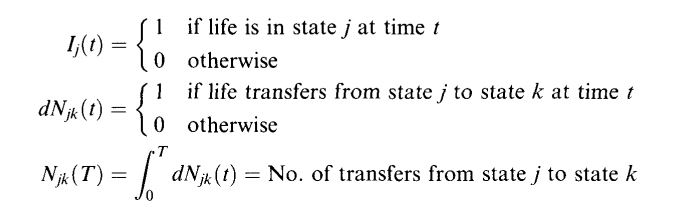
\includegraphics[width=10cm]{equation.JPG}
    \label{fig:Plot}
\end{figure} 

\item The mean age at onset of AD, given that the life was eventually institutionalised with AD.
\[E[x+\int_{x}^{w}I_1(t)dt | N_{23}(w-x) = 1\ and\ I_1(x) =1 ] = \]
\[=x + \frac{\int_{x}^{w}(t-x)\mu_t^{12}P_{xt}^{11}[\int_{x}^{w}\mu_{s}^{23}P_{ts}^{22}ds]dt}{\int_{x}^{w}\mu_t^{12}P_{xt}^{11}[\int_{x}^{w}\mu_s^{23}P_{ts}^{22}ds]dt }\]

\item The mean time from onset of AD to institutionalisation:
\[E[\int_{x}^{w}I_2(t)dt | N_{23}(w-x) = 1\ and\ I_1(x) =1 ] = \]
\[= \frac{\int_{x}^{w}\mu_t^{12}P_{xt}^{11}[\int_{x}^{w}(s-t)\mu_{s}^{23}P_{ts}^{22}ds]dt}{\int_{x}^{w}\mu_t^{12}P_{xt}^{11}[\int_{x}^{w}\mu_s^{23}P_{ts}^{22}ds]dt }\]

Here w denotes upper bound age which we took at 120 years age.
\\ Using the Gompertz approximation . Although it is appropriate to allow for future improvements in mortality in applications, it is not appropriate to do so in estimation based on past data. The values of constant do not depend strongly on the baseline mortality.
\[\mu_{x+t}^{12} = A +\mu_{x+t}^{AD} \]
\[\mu_{x+t}^{23} = D\]
\[\mu_{x+t}^{24} = P\mu_{x+t}^{14}\]
\[\mu_{x+t}^{14} = AM\mu_{x+t}  \]
$\mu_{x+t}^{14}$baseline mortality, was taken as AM 80 mortality, using the Gompertz approximation.Here A,D and P is constant which we derive by extending  Gompertz approximation.   
SO, \[\mu_{x+t}^{jk}=A + DB\exp^{C(x+t)}\] 
\item  model the incidence of AD for the ith genotype as:
For use in our model, these odds ratios have to be converted into relative risks.transition intensities that are consistent with the odds ratios and together are consistent with the aggregate incidence of AD.
\[\mu_{x+t}^{i12} = r_1 f_{x+t}^{i}\mu_{x+t}^{AD} \]
\\where $f_{x+t}^{i}$ is a parametric function representing the relative risk. $f_{x+t}^{i}$  = 1 in the case of the $\epsilon$3/$\epsilon$3 genotype.
\\$\mu_{x+t}^{AD}$ is a aggregate incident rate of AD.
\\$r_1$ is a constant.
\item To determine the parameter $r_1$, we calculated the aggregate incidence of AD in the whole model, and fitted this to $\mu_{x+t}^{AD}$ by least square, If $ iP_{xt}^{11}$ is the probability that a life with genotype i, healthy at age x, is unaffected by AD at age x + t,and if $P_i^x$ is the population frequency of the ith genotype at age x then the aggregate incidence of AD 

aggregation intensity at x+t = $r_1 \big\{\sum_{n=1}^{5}P_x^{i}P_{xt}^{11f_{x+t}^{i}}\big\} \mu_{x+t}^{AD} $
\item To allow for this possibility we will also consider models assuming that the true relative risks are a proportion $m<1$ of those estimated above. We do this by adjusting equation  so that for genotype i:
\[\mu_{x+t}^{i12}=r_m[(f_{x+t}^{i} - 1)m + 1]\mu_{x+t}^{AD}  \] 
Here, $r_m$  is chosen as above so that the aggregate incidence of AD in the model is consistent with $\mu_{x+t}^{AD}$





\end{itemize}



\section{Pseudo Code/ Algorithm }

\begin{itemize}
    \item Pseudo Code for Figure 2\\
    begin \\
    declare x1 from 65 to 120\\
calculate y1 equal from  the formula ($10^{-5}$)*9.4116 * exp(0.084554 * x1  )\\
declare x2 from 65 to 120\\
calculate y2 from the formula ($10^{-5}$)*2.593 * exp(0.084554 * x2  )\\
plot(x1,y1,x2,y2)\\
end\\
\item Pseudo Code for Figure 3\\
begin\\
declare x from 40 to 90\\
assign E1 equal to 2.98\\
assign F1 equal to 0.00312 \\
assign G1 equal to 0\\
assign H1 equal to 1\\
assign k11 equal to 62\\
assign k12 equal to 0\\
assign P1 equal  to exp(-F1 .* ($(x-k11).^2$) - G1.*(x-k12)) \\
assign fi1 equal to  E1 .* P1 + H1 \\
assign E2 equal to 13.5\\
assign F2 equal to 0.00529\\
assign G2 equal to 0\\
assign H2 equal to 1\\
assign k21 equal to 60\\
assign k22 to 0\\
assign P2 equal to exp(-F2 .* ($(x-k21).^2$) - G2.*(x-k22))\\
assign fi2 equal to E2 .* P2 + H2\\

assign E3 equal to 2.87\\
assign F3 equal to 0.00938\\
assign G3 equal to 0\\
assing H3 equal to 1\\
assign k31 equal to 68\\
assign k32 equal to 0\\

assign P3 equal to exp(-F3 .* ($(x-k31).^2$) - G3.*(x-k32))\\
assign fi3  E3 .* P3 + H3 \\
assign E4 0.754 \\
assign F4 equal to 0\\
assign G4 equal to 0.00859 \\
assign H4 equal to 0\\
assign k41 equal to 0 \\
assign k42 equal to 60 \\
assign P4 equal to exp(-F4 .* ($(x-k41).^2$) - G4.*(x-k42));\\
assign fi4 equal to E4 .* P4 + H4 \\
plot(x,fi1,x,fi2,x,fi3,x,fi4)\\
end\\
\end{itemize}
\section{Coding and Simulation} 
\subsection{Simulation Framework}
$f_{x+t}^{i}$ is a parametric function representing the risk relative to the aggregate incidence rate.
\begin{align*}
 f_{x+t}^{i} = E \exp^{-F((x+t)-k2)^2 -((x+t)-k2)}+H   
\end{align*}
\newline
By considering the form of the OR, we set either F = 0 for giving an exponential function or G = 0  for giving a bell-curve function.
\newline
Value of k1 or k2 is the nearest integer by inspection.
\newline
Whole result dependent is odd rations, they are controlling parameters of the all result.

\newpage
\subsection{Reproduced Figures}
\begin{itemize}
\item Used Tools (MATLAB)
\item Reproduced Figures
    \begin{figure}[htp]
    \centering
    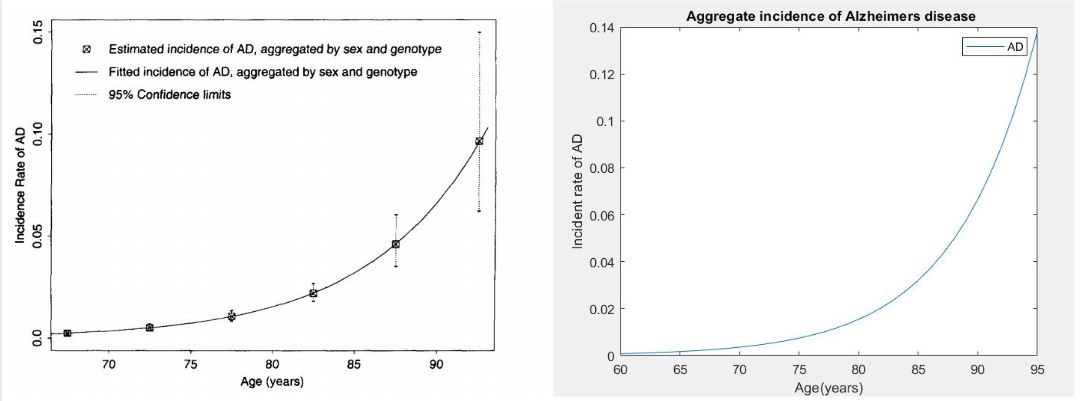
\includegraphics[width=17cm]{fig2.JPG}
    \caption{Aggregate incidence of Alzheimer's disease}
    \label{fig:Plot}
\end{figure}

    \begin{figure}[htp]
    \centering
    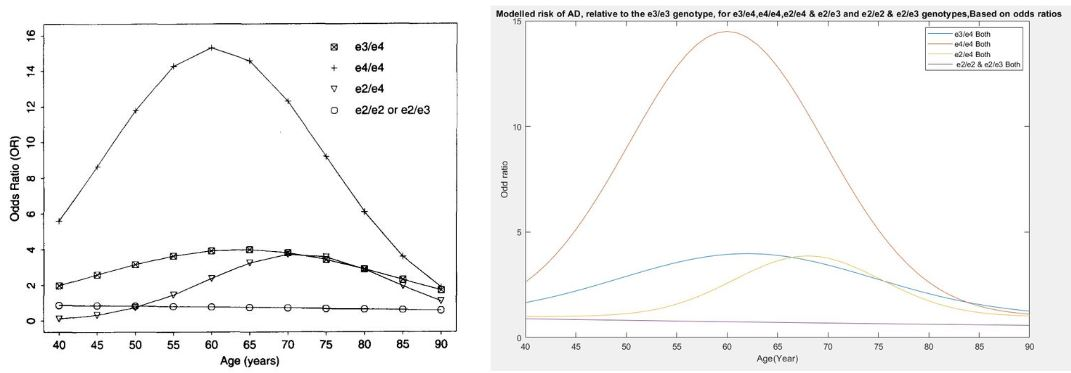
\includegraphics[width=17cm]{fig3.JPG}
    \caption{Odds ratios (ORs) of AD relative to $\epsilon$1/$\epsilon$3 genotype for males and females combined.}
    \label{fig:Plot}
\end{figure}
    \begin{figure}[htp]
    \centering
    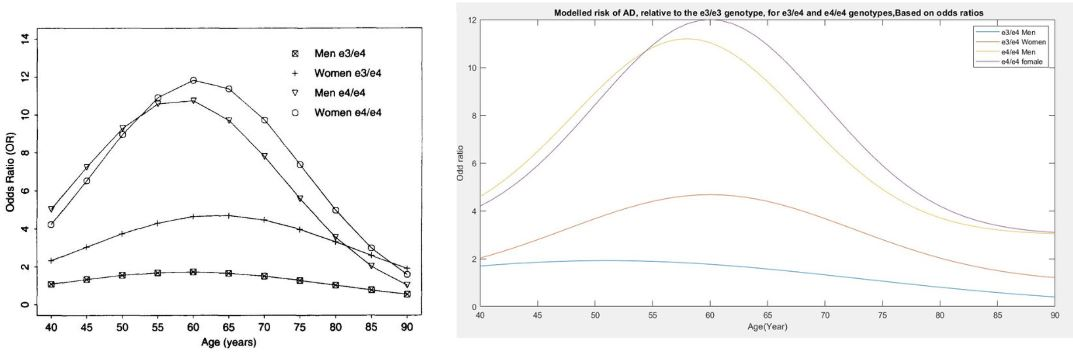
\includegraphics[width=17cm]{fig4.JPG}
    \caption{Odds ratios (ORs) of AD relative to $\epsilon$3/$\epsilon$3 genotype for $\epsilon$3/$\epsilon$4 and $\epsilon$4/$\epsilon$4 genotypes}
    \label{fig:Plot}
\end{figure}
    \begin{figure}[htp]
    \centering
    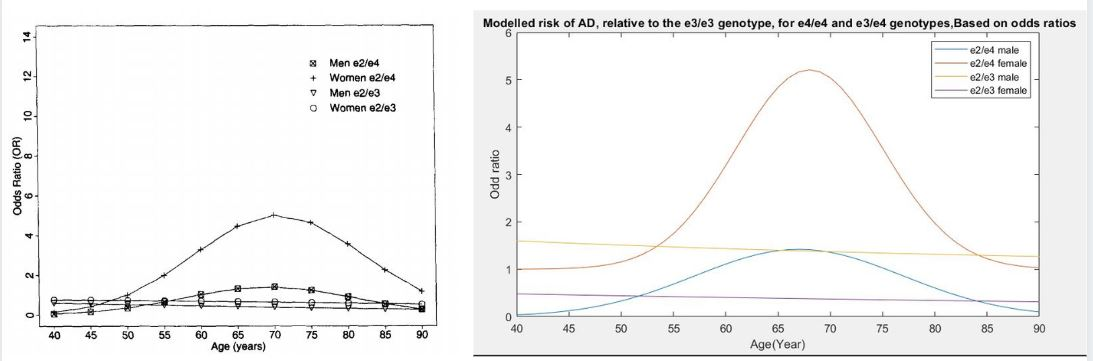
\includegraphics[width=17cm]{fig5.JPG}
    \caption{Odds ratios (ORs) of AD relative to $\epsilon$3/$\epsilon$3 genotype for $\epsilon$2/$\epsilon$2 or $\epsilon$2/$\epsilon$3 and $\epsilon$2/$\epsilon$4 genotypes.}
    \label{fig:Plot}
\end{figure}
    \begin{figure}[htp]
    \centering
    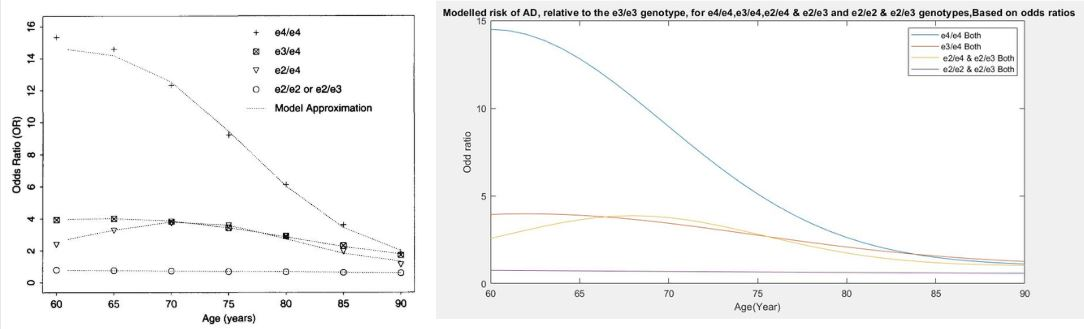
\includegraphics[width=17cm]{fig6.JPG}
    \caption{Odds ratios (ORs) of AD relative to $\epsilon$3/$\epsilon$3 genotype, compared with ORs
computed using modelled relative risk functions.}
    \label{fig:Plot}
\end{figure}
    \begin{figure}[htp]
    \centering
    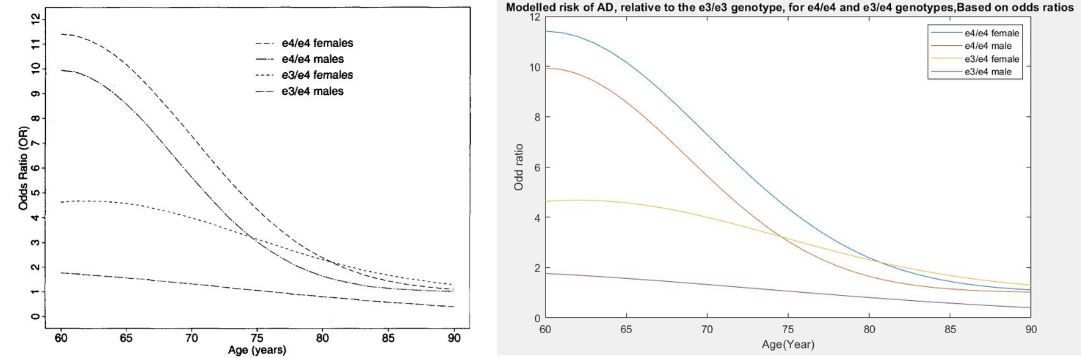
\includegraphics[width=17cm]{fig7.JPG}
    \caption{Modelled risk of AD, relative to the $\epsilon$3/$\epsilon$3 genotype, for $\epsilon$4/$\epsilon$4 and $\epsilon$3/$\epsilon$4 genotypes. Based on
odds ratios}
    \label{fig:Plot}
\end{figure}
    \begin{figure}[htp]
    \centering
    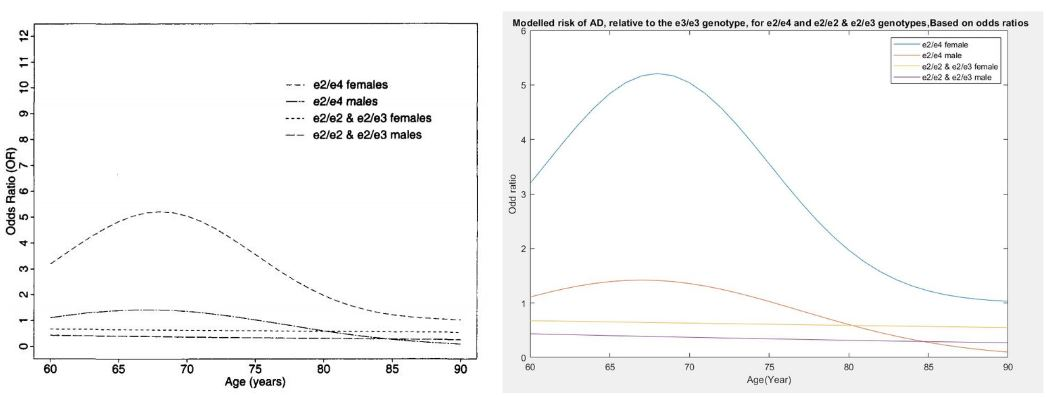
\includegraphics[width=17cm]{fig8.JPG}
    \caption{Modelled risk of AD, relative to the $\epsilon$3/$\epsilon$3 genotype, for $\epsilon$2/$\epsilon$4 and $\epsilon$2/$\epsilon$2 & $\epsilon$2/$\epsilon$3 genotypes. Based on odds ratios}
    \label{fig:Plot}
\end{figure}
    \begin{figure}[htp]
    \centering
    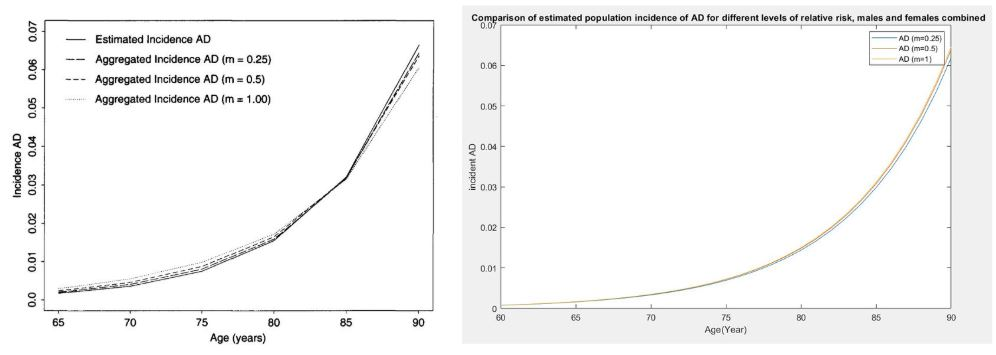
\includegraphics[width=17cm]{fig9.JPG}
    \caption{Comparison of estimated population incidence of AD $\mu^{AD}_{x+t}$, with the aggregated incidence of AD for different levels of relative risk, males and females combined.}
    \label{fig:Plot}
\end{figure}
\end{itemize}
\newpage

\begin{itemize}
\subsection{New Work Done}

\subsubsection{New Analysis}
\item A simple model of Alzheimer's disease,which preditct the probablity of changing the states
\item Assumption:-
\newline
(1)All states are independent of each other.
\newline
(2)All makehom constants are independent to each other.
\newline
(3)D and P are not dependent on $\mu_{x+t}^{AM80}$ and A is a nuisance parameter.
\newline
(4)Here j is a lower limit which is 60 and w is a upper limit which is 95 in our case. 
\newline
\[{AM80}\mu_{x+t} = 0.000094116\exp^{0.084554(x+t)}\]
\[\mu_{x+t}^{AD}=1.31275\times 10^{-7}\times\exp^{0.1459(x+t)} \]
\[\mu_{x+t}^{12} = A +\mu_{x+t}^{AD} \]
\[\mu_{x+t}^{23} = D\]
\[\mu_{x+t}^{24} = P\mu_{x+t}^{14}\]
\[\mu_{x+t}^{14} = AM80\mu_{x+t}  \]
\[Transition Intensity =\int_{j}^{w} \mu_{x+t}^{12} \mu_{x+t}^{23} \mu_{x+t}^{24} \mu_{x+t}^{14}dt \]
\[= \int_{j}^{w} (A +\mu_{x+t}^{AD})D(P\mu_{x+t}^{14})(AM80\mu_{x+t})dt \]
\[= \int_{j}^{w}DP(AM80\mu_{x+t}^{24})dt + \int_{j}^{w}DP(AM80\mu_{x+t}) \mu_{x+t}^{14}dt\]
\newline
\newline
\item Probability of changing state from No Alzheimer to on set Alzheimer for different genotype
\newline
(1)$f_{x+t}^{i}$ is parametric function representing the risk relative to the
aggregate incidence rate.
\newline
(2) $r_i$ is a constant chosen so that the aggregate incidence of AD based on the modelled intensities is consistent with the aggregate incidence
\newline
(3)Here j is a lower limit which is 60 and w is a upper limit which is 95 in our case.
\newline
\[\mu_{x+t}^{AD}=1.31275\times 10^{-7}\times\exp^{0.1459(x+t)} \]
\[f_i = E \exp^{-F((x+t)-k2)^2 -((x+t)-k2)}+H \]
\[\mu_{x+t}^{i12} = r_1 f_{x+t}^{i}\mu_{x+t}^{AD} \]
\[= \int_{j}^{w}\mu_{x+t}^{i12}dt\] 
\[= \int_{j}^{w} r_1 f_{x+t}^{i}\mu_{x+t}^{AD} dt  \]
\[= \int_{j}^{w}r_1(E \exp^{-F((x+t)-k2)^2 -((x+t)-k2)}+H)1.31275\times 10^{-7}\times\exp^{0.1459(x+t)} \]
\newpage
\subsubsection{New Results}
\begin{figure}[htp]
    \centering
    \includegraphics[width=17cm]{new1stateschange.JPG}
    \caption{A simple model of Alzheimer's disease,which preditct the probablity of changing the states}
    \label{fig:Plot}
\end{figure}
\begin{figure}[htp]
    \centering
    \includegraphics[width=17cm]{new2u12.JPG}
    \caption{Probability of changing state from No Alzheimer to on set Alzheimer for different genotype}
    \label{fig:Plot}
\end{figure}
\begin{figure}[htp]
    \centering
    \includegraphics[width=17cm]{new3u23.JPG}
    \caption{A simple model of Alzheimer's disease,which preditct the probablity of changing the states}
    \label{fig:Plot}
\end{figure}
\begin{figure}[htp]
    \centering
    \includegraphics[width=17cm]{new4u24.JPG}
    \caption{Probability of changing state from Institutionalised Alzheimer to Death for different genotype}
    \label{fig:Plot}
\end{figure}
\begin{figure}[htp]
    \centering
    \includegraphics[width=17cm]{new5u34.JPG}
    \caption{A simple model of Alzheimer's disease,which preditct the probablity of changing the states}
    \label{fig:Plot}
\end{figure}
\end{itemize}

\newpage
\subsubsection{New Inferences}
\begin{itemize}
    \item A simple model of Alzheimer's disease,which preditct the probablity of changing the states
    \newline
    By the Fig.10, We conclude that probability of any person who has Alzheimer.He/She is in onset Alzheimer state then their chances of moving from onset Alzheimer to to die is higher than on set Alzheimer to institutionalised Alzheimer for every age.That shows that more peoples die after on set Alzheimer than going to institutionalised Alzheimer state.
     \item  We can see that transition from onset Alzheimer to institutionalised is constant throughout all ages.
    \item Transition from no Alzheimer to Institutionalised Alzheimer is low through initial age(till age of 80) and after that it will increases exponentially.So the chances for getting Alzheimer is high after the age of 80 years. 
    \newline
    \newline
    \item Probability of changing state from No Alzheimer to on set Alzheimer for different genotype
    \item If we further describe No Alzheimer to On set Alzheimer in terms of genes,Because The peoples who has any combination with E4 genes has higher chances of getting affected by Alzheimer.
    \item So,We analysed that peoples who have combination of e2 and e4 genes(e2/e4) has lowest chances of getting affected by Alzheimer. Which shows that e2 allele gene work against e4 allele gene.And which shows that e2 allele genes helps peoples for recovering the Alzheimer.
    \item After the initial age (Age of 85 years) e3/e4 combination has high probability to getting affected with Alzheimer then e4/e4 genes.Which shows us that e3 allele gene with combination of e4 allele gene is more influenced factor then e4/e4 gene.
    \newline
    \newline
    \item Probability of changing state to Institutionalised from onset Alzheimer for different genotype
    \item If we analyse the fig.12 we clearly see the transition from on set Alzheimer to die($\mu_{x+t}^{i24}$), in which male are affected more than female. After initial age it will increases exponential.
    \newline
    \newline
    \item Probability of changing state from Institutionalized Alzheimer to Death for different genotype.
    \item If we analyse the fig.13 we clearly see the transition from institutionalised  Alzheimer to die($\mu_{x+t}^{i34}$), in which male are affected more than female. After initial age it will increases exponential.    
\end{itemize}

\section{ Contribution of team members}	



\subsection{Technical contribution of all team members. }
\begin{table}[h]
\centering
\begin{tabular}{|l|l|l|}
\hline
Tasks  & Parth Patel & Shivam Lakhtariya \\ \hline
Modeling &    Done           &    Done          \\ \hline
Coding &    Done           &    Done      \\ \hline
Inference &    Done           &    Done          \\ \hline
\end{tabular}
\end{table}
\subsection{Non-Technical contribution of all team members }
Enlist the non-technical contribution of members in the table. Redefine the tasks (e.g Task-1 as report writing etc.)
\begin{table}[h]
\centering
\begin{tabular}{|l|l|l|}
\hline
Tasks  & Parth Patel & Shivam Lakhtariya\\ \hline
Mathematical Work &    Done           &    Done          \\ \hline
Report Writing &    Done           &    Done          \\ \hline
C Map &    Done           &    Done          \\ \hline
Inferences & Done  & Done       \\ \hline
\end{tabular}
\end{table}

\bibliographystyle{IEEEtran}
\bibliography{ref.bib}

\end{document} 